
\documentclass{article}
\usepackage[utf8]{inputenc}
\usepackage{amsmath}
\usepackage{amssymb}
\usepackage{amsbsy}
\usepackage{graphicx}
\usepackage{xspace}
\setcounter{secnumdepth}{-1}

%% notation
% I nearly called this 'smartmath', but am anticipating feeling really stupid for thinking this was smart in half a year or so
\newcommand{\mathspace}[1]{\ensuremath{#1}\xspace} %command for defining commands

% differential operators and such
\newcommand{\D}{\mathspace{\mathbf{D}}}
\newcommand{\sigmabf}{\mathspace{\boldsymbol{\sigma}}}
\newcommand{\grad}{\mathspace{\nabla}}
\renewcommand{\div}{\mathspace{\nabla \cdot}}
\newcommand{\inner}[2]{\mathspace{\left (#1, #2 \right)}}
\newcommand{\defeq}{\mathspace{:=}}
% \newcommand{\ddt}[1]{\mathspace{\frac {\partial #1} {\partial t}}}
\newcommand{\ddt}[1]{\mathspace{\partial_t #1}}
\newcommand{\dt}{\mathspace{\Delta t}}

% domains and normals
\newcommand{\taubf}{\mathspace{\boldsymbol{\tau}}}
\newcommand{\stokes}{\mathspace{\Omega_{f}}}
\newcommand{\stokesbdy}{\mathspace{\Gamma_{f}}}
\newcommand{\darcy}{\mathspace{\Omega_{p}}}
\newcommand{\darcybdy}{\mathspace{\Gamma_{p}}}
\newcommand{\interface}{\mathspace{\Gamma_{fp}}}
\newcommand{\nf}{\mathspace{\mathbf{n}_f}}
\newcommand{\np}{\mathspace{\mathbf{n}_p}}

% shorthands for integrals - i.e. integral over Stokes, Stokes bdy + interface, Stokes bdy, interface
\newcommand{\intD}{\mathspace{\int \limits_{\darcy}}}
\newcommand{\intDbdyI}{\mathspace{\int \limits_{\partial \darcy}}}
\newcommand{\intDbdy}{\mathspace{\int \limits_{\darcybdy}}}
\newcommand{\intS}{\mathspace{\int \limits_{\stokes}}}
\newcommand{\intSbdyI}{\mathspace{\int \limits_{\partial \stokes}}}
\newcommand{\intSbdy}{\mathspace{\int \limits_{\stokesbdy}}}
\newcommand{\intI}{\mathspace{\int \limits_{\interface}}}


% fluid test\trial functions


\newcommand{\uf}{\mathspace{\mathbf{u}_f}}
\newcommand{\vf}{\mathspace{\mathbf{v}_f}}
\newcommand{\up}{\mathspace{\mathbf{u}_p}}
\newcommand{\vp}{\mathspace{\mathbf{v}_p}}

% pressure test\trial functions
\newcommand{\pf}{\mathspace{p_f}}
\newcommand{\pp}{\mathspace{p_p}}
\newcommand{\wf}{\mathspace{w_f}}
\renewcommand{\wp}{\mathspace{w_p}}

% displacement test\trial functions
\newcommand{\disp}{\mathspace{\boldsymbol{\eta}_p}}
\newcommand{\disptest}{\mathspace{\boldsymbol{\xi}_p}}

% multiplier test\trial functions
\newcommand{\mult}{\mathspace{\lambda_{\Gamma}}}
\newcommand{\multtest}{\mathspace{\mu_{\Gamma}}}



\begin{document}

\title{Equations for system}
\maketitle


We follow \cite{ambartsumyan} very very closely.

\section{Domain}
Our domain $\Omega$ is $d=2 \text{ or } 3$-dimensional, and partitioned into \stokes and \darcy, with $\interface = \stokes \cap \darcy$ being the $(d-1)$-dimensional interface. The boundary $\partial \Omega$ is partitioned into $\stokesbdy = \partial \Omega \cap \partial \stokes$ and $\darcybdy = \partial \Omega \cap \partial \darcy$. We assume each region is connected, reasonably smooth and all that.

\section{Unknowns}
The unknowns of the system and the corresponding test functions are:

\begin{itemize}
\item \uf, \vf : free flow fluid velocity. Defined on \stokes.
\item \up, \vp : porous flow fluid velocity. Defined on \darcy.
\item \pf, \wf : free flow fluid pressure. Defined on \stokes.
\item \pp, \wp : porous flow fluid pressure. Defined on \darcy.
\item \disp, \disptest : displacement. Defined on \darcy.
\item \mult, \multtest : normal stress balance Lagrange multiplier. Defined on \interface. In \cite{ambartsumyan}, denoted $\lambda, \mu_h$.

\end{itemize}

\section{Parameters}

\begin{description}
\item[$\mu_f$] fluid viscosity (denoted $\mu$ in the \cite{ambartsumyan})
  
\item[$\lambda_p, \mu_p$] Lamé parameters. Denoted $\mu$ in \cite{ambartsumyan}.
\item[$\alpha$] Biot-Willis constant
\item[$K$] Permeability tensor. Symmetric, bounded, positive definite. I take it to be scalar.
\item[$\alpha_{BJS}$] Friction coefficient
\item[$s_0$] Storage coefficient
\item[$B=$] $\frac {\mu_f \alpha_{BJS}} {\sqrt{K}}$ The coefficient in the BJS condition. Could be zero.
\end{description}

\section{Notation}
\begin{itemize}
\item \nf, \np are the outward unit normal vectors to $\partial \stokes, \partial \darcy$. 
\item $\taubf_{f, j}, j = 1, \ldots, d-1$ is an orthogonal system of unit tangent vectors at \interface.
\item $\D(\mathbf{v}) \defeq \frac 12 (\grad \mathbf{v} + \grad \mathbf{v}^T)$
\item $\sigmabf_f(\uf, \pf) \defeq -\pf \mathbf{I} + 2 \mu_f \D(\uf)$
\item $\sigmabf_p(\disp, \pp) \defeq \lambda_p (\div \disp)\mathbf{I}  + 2 \mu_p \D(\disp) - \alpha \pp \mathbf{I} $
\end{itemize}

Next, here are a bunch of bilinear forms used in the problem: 
\begin{itemize}
\item $a_f(\uf, \vf) = \inner{2\mu \D(\uf)} {\D(\vf)}_{\stokes}$
\item $a_p^d(\up, \vp) = \inner{\mu K^{-1}\up} {\vp}_{\darcy}$
\item $a_p^e(\disp, \disptest) = \inner{\mu_p \D(\disp)} {\D(\disptest)}_{\darcy} + \inner{\lambda_p \div \disp} {\div \disptest}_{\darcy}$
\item $b_f(\vf, \wf) = -\inner{\div \vf}{\wf}_{\stokes}$
\item $b_p(\vp, \wp) = -\inner{\div \vp}{\wp}_{\darcy}$
  
\item $a_{BJS}(\uf, \disp; \vf, \disptest) = \frac {\mu \alpha_{BJS}} {\sqrt{K}} \sum_{j=1}^{d-1} \inner{(\uf - \disp) \cdot \taubf_j}{ (\vf - \disp) \cdot \tau_j}_{\interface} $
\item $b_{\interface}(\vf, \vp, \disptest; \multtest) = \inner{\vf \cdot \nf + (\disptest + \vp) \cdot \np}{\multtest}_{\interface}$
  
\end{itemize}


\section{Strong formulation}
These are all ignoring body force and source terms. So it's okay to put stuff on the right hand sides if you want to.

Stokes (applies in \stokes):
\begin{subequations}
  \begin{align}
    - \div \sigmabf_f (\uf, \pf) = 0    \label{eq:stokes_stress} \\
    \div \uf = 0    \label{eq:stokes_conservation}
  \end{align}
\end{subequations}

Darcy (applies in \darcy):
\begin{equation}
    \up = - \frac {K} {\mu} \grad \pp     \label{eq:darcy}
  \end{equation}

  
Biot (applies in \darcy):
\begin{subequations}
  \begin{align}
    - \div \sigmabf_p (\disp, \pp) = 0     \label{eq:biot_stress} \\
    \ddt{} \left ( s_0 \pp + \alpha \div \disp \right ) + \div \up = 0    \label{eq:biot_conservation}
  \end{align}
\end{subequations}
\section{Interface conditions}

Conservation of mass:
\begin{equation}
\uf  \cdot \nf + \left ( \ddt{\disp} + \up \right ) \cdot \np = 0  \label{eq:massconservation}
\end{equation}
Balance of stress :
\begin{equation}
  -(\sigmabf_f \nf) \cdot \nf = \pp + C_p = \lambda  \label{eq:stressbalance1_mult}
\end{equation}
\begin{equation}
  \sigmabf_f \nf + \sigmabf_p \np = 0 \:  \label{eq:stressbalance2}
\end{equation}
BJS condition:
\begin{equation}
  -(\sigmabf_f \nf) \cdot \taubf_j = B \left ( \uf - \ddt{\disp} \right ) \cdot \taubf_j
  \label{eq:BJS}
\end{equation}


\cite{ambartsumyan} does not have the constant $C_p$ in (5), but their interface is 'actually flat' and not a vessel wall with muscles extering force of their own, so that's reasonable.


\section{Boundary conditions}
In their numerical experiment (section 7.2), \cite{ambartsumyan} use the domain shown in figure \ref{fig:ambartsumyandomain}
\begin{figure}[h]
  \centering
  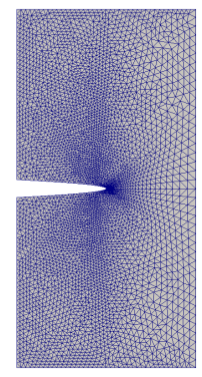
\includegraphics[width=0.15\textwidth]{img/ambartsumyandomain.png}
  \label{fig:ambartsumyandomain}
  \caption{Darcy domain from \cite{ambartsumyan}. Stokes domain is the removed 'finger'.}
\end{figure}
The Darcy boundary \darcybdy is partitioned into the left part $\darcybdy^{\text{L}}$ and the remainder $\darcybdy^{\neg \text{L}}$ in the obvious way. Physically, I think $\darcybdy^{\text{L}}$ is above ground and the other part is below ground or something.

As boundary conditions, they use:
\begin{itemize}
\item $\uf = 10 \nf$ on \stokesbdy
\item $\up \cdot \np = 0$ on $\darcybdy^{\text{left}}$
\item $\pp = 1000$ on $\darcybdy^{\neg \text{left}}$
\item $\disp \cdot \np = 0$ on $\darcybdy^{\neg \text{left}}$
\item $(\sigmabf_p \np) \cdot \taubf_p = 0$ on $\darcybdy^{\neg \text{left}}$

I think I can use essentially the same boundary conditions, although maybe I should prescribe the pressure on \stokesbdy instead of the flow.
 
\end{itemize}
\section{Variational formulation}
Having used a backward Euler discretization of the time derivative, \cite{ambartsumyan} obtain the following variational formulation

\begin{subequations}
  \begin{align}
    a_f(\uf, \vf) +& b_f(\vf, \pf)  + a^e_p(\disp, \disptest) \label{eq:varform1} \\
    +&\alpha b_p(\disptest, \pp)  + a_p^d(\up, \vp) + b_p(\vp, \pp)  \nonumber \\
    + &b_{\interface}\left (\vf, \vp, \disptest; \lambda \right ) + a_{BJS}\left (\uf, \frac{\disp} {\dt}; \vf, \disptest \right)\nonumber \\
                   = a_{BJS}\left (\uf, \frac{\disp^{n-1}} {\dt}; \vf, \disptest \right) + & \inner{\vp}{C_p\np}_{\interface} + (\sigmabf_f\nf, \vf)_{\stokesbdy} \nonumber \\
                   + & (\sigmabf_p\np, \disptest)_{\darcybdy} + (\pp\np, \vp)_{\darcybdy}\nonumber \\ \nonumber \\
    % a_f (\uf, \vf) &+ a_p^d(\up, \vp) + a_p^e(\disp, \disptest)  + a_{BJS}\left (\uf, \frac {\disp} {\dt}; \vf, \disptest \right) \label{eq:varform1} \\
    %                & + b_f(\vf, \pf) + b_p(\vp, \pp) + \alpha b_p(\disptest, \pp)   \nonumber \\
    %                & + b_{\interface}(\vf, \vp, \disptest; \mult) \nonumber \\
    %                &= a_{BJS}\left (\uf, \frac {\disp^{n-1}} {\dt}; \vf, \disptest \right)  + b_{\interface}(\vf, \vp, \disptest; C_p) \nonumber \\ 
    \inner{s_0 \frac {\pp} {\dt}}{\wp}_{\darcy}  &- \alpha b_p\left ( \frac{\disp} {\dt}, \wp \right ) - b_p(\up, \wp) - b_f(\uf, \wf) \label{eq:varform2}
    \\ = \inner{s_0 \frac {\pp^{n-1}} {\dt}}{\wp}_{\darcy} &- \alpha b_p\left ( \frac {\disp^{n-1}} {\dt}, \wp \right )_{\darcy}\nonumber \\ \nonumber \\
    b_{\interface}\left (\uf, \up, \disp; \multtest \right ) &= b_{\interface}\left (\uf, \up, \disp^{n-1}; \multtest \right ) \label{eq:varform3}
  \end{align}
\end{subequations}

Here the unknowns with no superscript mean the unknowns at time $n$ (e.g. $\uf = \uf^n$). 



\section{Derivation of weak form}
Briefly, \eqref{eq:varform1} is \eqref{eq:stokes_stress} multiplied by \vf integrated over \stokes; \eqref{eq:biot_stress} multiplied by \disptest integrated over \darcy; and \eqref{eq:darcy} multiplied \vp integrated over \darcy. The interface conditions are also all used.

To be more detailed, multiply \eqref{eq:stokes_stress} by \vf and integrate over \stokes. By standard vector calculus,
$$\intS - \vf \cdot \div \sigmabf_f = \intS \sigmabf_f \colon \grad \vf - \intSbdyI \sigmabf_f\nf  \cdot \vf.$$
Now, as the $\partial \stokes$ consists of \stokesbdy and \interface, the boundary term splits into an integral over \stokesbdy which we can move to the RHS by applying boundary conditions \footnote{Specifically, Dirichlet conditions on \uf or Neumann conditions on $\sigmabf_f$.}, and an interface term $-I_{\vf} = -\intI \sigmabf_f \nf \cdot \vf$.

Before proceeding, we expand\footnote{The equality $\D(\uf) \colon \grad \vf = \D(\uf) \colon \D(\vf)$ looks false because $\grad \vf \neq \D(\vf)$, but $\D(\uf)$ is symmetric, so $\D(\uf) \colon \grad \vf = \D(\uf) \colon \grad \vf^T = \D(\uf) \colon \D(\vf)$.}
\begin{align*}
  \intS \sigmabf_f \colon \grad \vf &= \intS (-\pf \mathbf{I} + 2 \mu_f \D(\uf)) \colon \grad \vf \\
                                    &= \intS -\pf \div \vf + \intS 2 \mu_f \D(\uf) \colon \grad \vf \\
                                      &= b_f(\vf, \pf) + a_f(\uf, \vf)
\end{align*}
So the contribution here is $$a_f(\uf, \vf) + b_f(\vf, \pf) -I_{\vf} - (\sigmabf_f\nf, \vf)_{\stokesbdy}.$$


% Next, multiply \eqref{eq:stokes_conservation} by \wf and integrate over \stokes. This becomes
% $$\intS \wf \cdot \div \uf = $$

Next, multiply \eqref{eq:biot_stress} by \disptest and integrate over \darcy. By exactly the same argument,
$$\intD - \disptest \cdot \div \sigmabf_p = \intD \sigmabf_p \colon \grad \disptest - \intDbdyI \sigmabf_p\np  \cdot \disptest.$$

Again, the boundary term splits into an integral over \darcybdy where we need boundary conditions \footnote{Specifically, Dirichlet conditions on \disp or Neumann conditions on $\sigmabf_p$.} and an interface term $-I_{\disptest} = -\intI \sigmabf_p \np \cdot \disptest$. Expanding,

\begin{align*}
  \intD \sigmabf_p \colon \grad \disptest &=  \intD  \left ( \lambda_p (\div \disp)(\div \disptest)  + 2 \mu_p \D(\disp) \colon \grad \disptest \right)
                                            - \alpha \pp \div \disptest \\
                                          &= a^e_p(\disp, \disptest) + \alpha b_p(\disptest, \pp)
\end{align*}
So the contribution is $$a^e_p(\disp, \disptest) + \alpha b_p(\disptest, \pp) - I_{\disptest} - (\sigmabf_p\np, \disptest)_{\darcybdy}.$$

Next, multiply \eqref{eq:darcy} by $\frac {\mu} {K} \vp$ and integrate over \darcybdy. Integration by parts yields
$$ \intD \frac {\mu} {K} \vp \cdot \uf -  \intD \pp \div \vp = \intDbdyI \pp \vp \cdot \np$$ 
The boundary term splits into an integral over \darcybdy where we need boundary conditions \footnote{Specifically, Dirichlet conditions on \up or Neumann conditions on \pp.} and an interface term $I_{\vp} = \intI \pp \vp \cdot \np$, so the contribution is
$$a_p^d(\up, \vp) + b_p(\vp, \pp) + I_{\vp} - (\pp \np, \vp)_{\darcybdy}.$$

Next, once we add all these equations together, we will have to handle the sum of the interface terms $$-I_{\vf} - I_{\disptest} + I_{\vp} = -\intI \sigmabf_f \nf \cdot \vf -\intI \sigmabf_p \np \cdot \disptest + \intI \pp \vp \cdot \np$$

We start with $\intI \pp \vp \cdot \np$. By \eqref{eq:stressbalance1_mult}, $\pp = \mult - C_p$ on \interface, so
$$I_{\vp} = \intI \pp \vp \cdot \np = \intI \mult \vp \cdot \np - \intI C_p \vp \cdot \np$$

The second term can then go live on the right hand side. Next, we treat the other two interface terms. By \eqref{eq:stressbalance2}, $\sigmabf_f \nf = - \sigmabf_p \np$, so we have that $$I_{\vf} + I_{\disptest} = \intI (\vf - \disptest) \cdot \sigmabf_f \nf$$
Next, note that the BJS condition \eqref{eq:BJS} gives us information on the tangential component of $\sigmabf_f \nf$, while \eqref{eq:stressbalance1_mult} gives us information on the normal component. As $\nf, \taubf_1, \taubf_2$ form an orthonormal system, we have that\footnote{This is just use of the fact when a vector $\mathbf{v}$ is written in a basis $\mathbf{e}_i$, the coefficient of $\mathbf{e}_i$    }
\begin{align*}
  \vf - \disptest = \: &\nf ((\vf - \disptest) \cdot \nf) + \sum_j \taubf_j ((\vf - \disptest) \cdot \taubf_j) \\
  \Longrightarrow \hspace{0.02\textwidth}  (\sigmabf_f \nf) \cdot (\vf - \disptest) = & \: ((\sigmabf_f \nf) \cdot \nf) \: ((\vf - \disptest) \cdot \nf) \\
  & + \sum_j ((\sigmabf_f \nf) \cdot \taubf_j) ((\vf - \disptest) \cdot \taubf_j)
\end{align*}
By \eqref{eq:stressbalance1_mult}, $(\sigmabf_f \nf) \cdot \nf = -\lambda$, and by \eqref{eq:BJS}, $(\sigmabf_f \nf) \cdot \taubf_j = -B \left ( \uf - \ddt{\disp} \right ) \cdot \taubf_j$, so

\begin{align*}
(\sigmabf_f \nf) \cdot (\vf - \disptest) =  \: &-\lambda\:  ((\vf - \disptest) \cdot \nf) \\
  &- \sum_j \left (B \left ( \uf - \ddt{\disp} \right ) \cdot \taubf_j \right ) ((\vf - \disptest) \cdot \taubf_j)
\end{align*}

We can then use that $\nf = - \np$ to write $\lambda \: (\vf - \disptest) \cdot \nf = \lambda \: (\vf  \cdot \nf + \disptest \cdot \np)$.
Putting it all together,

\begin{align*}
  -(I_{\vf} + I_{\disptest}) + I_{\vp}  =& \intI \lambda\: (\vf  \cdot \nf + (\disptest + \vp) \cdot \np) \\
  + &\intI \left (B \left ( \uf - \ddt{\disp} \right ) \cdot \taubf_j \right ) ((\vf - \disptest) \cdot \taubf_j) \\
  - &\intI C_p \vp \cdot \np \\
  = b_{\interface}\left (\vf, \vp, \disptest; \lambda \right ) & + a_{BJS}\left (\uf, \ddt{\disp}; \vf, \disptest \right) - \inner{\vp}{C_p\np}_{\interface} \\
\end{align*}

We have now derived all the necessary identities, and summing them all yields the following:
\begin{align*}
  a_f(\uf, \vf) +& b_f(\vf, \pf)  + a^e_p(\disp, \disptest)  \\ +&\alpha b_p(\disptest, \pp)  + a_p^d(\up, \vp) + b_p(\vp, \pp)  \\
  + &b_{\interface}\left (\vf, \vp, \disptest; \lambda \right ) + a_{BJS}\left (\uf, \ddt{\disp}; \vf, \disptest \right)\\
      = \inner{\vp}{C_p\np}_{\interface} +& (\sigmabf_f\nf, \vf)_{\stokesbdy} + (\sigmabf_p\np, \disptest)_{\darcybdy} + (\pp\np, \vp)_{\darcybdy}\\
\end{align*}

If \ddt{\disp} is now discretized by a backward Euler difference, this is exactly \eqref{eq:varform1}.

The next two are not as bad. \eqref{eq:varform2} is just \eqref{eq:stokes_conservation} multiplied by \wf integrated over \stokes plus \eqref{eq:biot_conservation} multiplied by \wp integrated over Darcy.

Doing the above (no integration of parts needed) yields

$$s_0\inner{\ddt{\pp}}{\wp}_{\darcy} - \alpha b_p(\ddt{\disp}, \wp)
- b_p(\up, \wp) - b_f(\uf, \wf)$$ 

Once the \ddt{}'s are discretized by a backward Euler difference, this is exactly \eqref{eq:varform2}.

Finally, \eqref{eq:varform3} is obtained by taking \eqref{eq:massconservation}, multiplying by \multtest and integrating over \interface. This yields $$b_{\interface} (\uf, \up, \ddt{\disp} ;\multtest) = 0$$
which, when \ddt{\disp} is discretized using a Backward Euler difference, yields \eqref{eq:varform3}.







\section{Thoughts}
\begin{itemize}
\item Kent offered very gentle scepticism about using a 3-field formulation, and suggested not having \up as an unknown, using $\up = \grad \pp$ to remove it. I thought \cite{ambartsumyan} had some opinion on this, but on closer reading I can't find it, so maybe that's from another article. I should read up on this.

\item Why is there a 2 in front of $\mu$ in equation \eqref{eq:stokes_stress}? If $\mu$ is just divided by 2 that's fine, but then I need to divide my choice by $\mu$ accordingly.

   
 
\end{itemize}


\bibliographystyle{amsalpha}
\begin{thebibliography}{99}
\bibitem{ambartsumyan}
{\sc Ambartsumyan, Ilona, et al. }, {\em "A Lagrange multiplier method for a Stokes-Biot fluid-poroelastic structure interaction model." }, arXiv preprint arXiv:1710.06750 (2017).
  
\end{thebibliography}

\end{document}
